\chapter{Co-segmentation based cell tracking} \label{chpt:coseg}
Cell tracking is an important method to quantitatively analyze time-lapse microscopy data. While numerous methods and tools exist for tracking cells in 2D time-lapse images, only few and very application-specific tracking tools are available for 3D time- lapse images, which is of high relevance in immunoimaging, in particular for studying the motility of microglia in vivo.

We introduce a novel algorithm for tracking cells in 3D time-lapse microscopy data, based on computing cosegmentations between component trees representing individual time frames using the so-called tree-assignments. For the first time, our method allows to track microglia in three dimensional confocal time-lapse microscopy images. We also evaluate our method on synthetically generated data, demonstrating that our algorithm is robust even in the presence of different types of inhomogeneous background noise.

Parts of this chapter follow closely the presentation from \cite{Xiao:2011}, where results of this thesis have been published.

\section{Introduction}

Capturing the motility of cells using time-lapse microscopy has become
an important approach to understanding processes such as the cell
cycle \cite{Harder:09}, neuronal division and migration
\cite{Norden:09}, immune response \cite{Cahalan:08}, or the
development of cancer \cite{Ianzini:09}. Based on phase-contrast,
confocal, or two-photon microscopy, such \emph{live cell imaging}
protocols are now commonly established and corresponding equipment is
commonly available. This has triggered the need for computational
methods to quantitatively analyze time-lapse microscopy data. In this
context, identifying individual cells and tracking their identities
over time is one of the basic ingredients for computational
analysis. Hence, \emph{cell tracking} algorithms have attracted
considerable attention in recent years
\cite{Meijering:06,Miura:05}. Here, we introduce a novel algorithm
for cell tracking that allows to track cells, in particular zebrafish
microglia, in three dimensional two-photon image sequences over time.

The majority of cell tracking algorithms, as surveyed by
\cite{Meijering:06} or \cite{Miura:05}, deals with cell tracking in
2D over time. Methods range from linking cells identified in
individual frames using different segmentation approaches to
active-contour \cite{dufour2005segmenting,Shen:06,Sacan:08} or level-set
algorithms \cite{Mukherjee:04,Nath:06,Dzyubachyk:08,Li:08}. The
challenges imposed by the nature of the images to be analyzed lie in
phenomena such as cell divisions \cite{AlKofahi:06,Li:08b}, cells
entering or leaving the displayed area, or a large number of cells
that needs to be tracked simultaneously. In addition, cell tracking is
often complicated by background inhomogeneity, for instance due to
uneven illumination \cite{Leong:03}, and cells touching each
other. While these issues have been addressed extensively for tracking
cells in 2D, surprisingly few approaches have addressed cell tracking
in 3D. Besides naive thresholding approaches, there are only few
advanced approaches, such as the active-contour based method proposed
by \cite{dufour2005segmenting}. Recently, several authors
\cite{Jaensch:10,Kerekes:09} proposed reliable methods for tracking
centrosomes in \emph{C.elegans} embryos. Yet, these approaches are
tailored towards tracking small, bright, and circular objects which
e.g. resemble a Gaussian spot of a specific size. Such assumptions,
however, are not satisfied by the complex and highly variable shapes
of microglia under consideration here. Cell tracking is also relevant
in the context of tracking cell populations \textit{in vitro}, which
has attracted considerable attention recently
\cite{House:09,Padfield:09,Ong:10}.

\begin{figure}
  \centering
  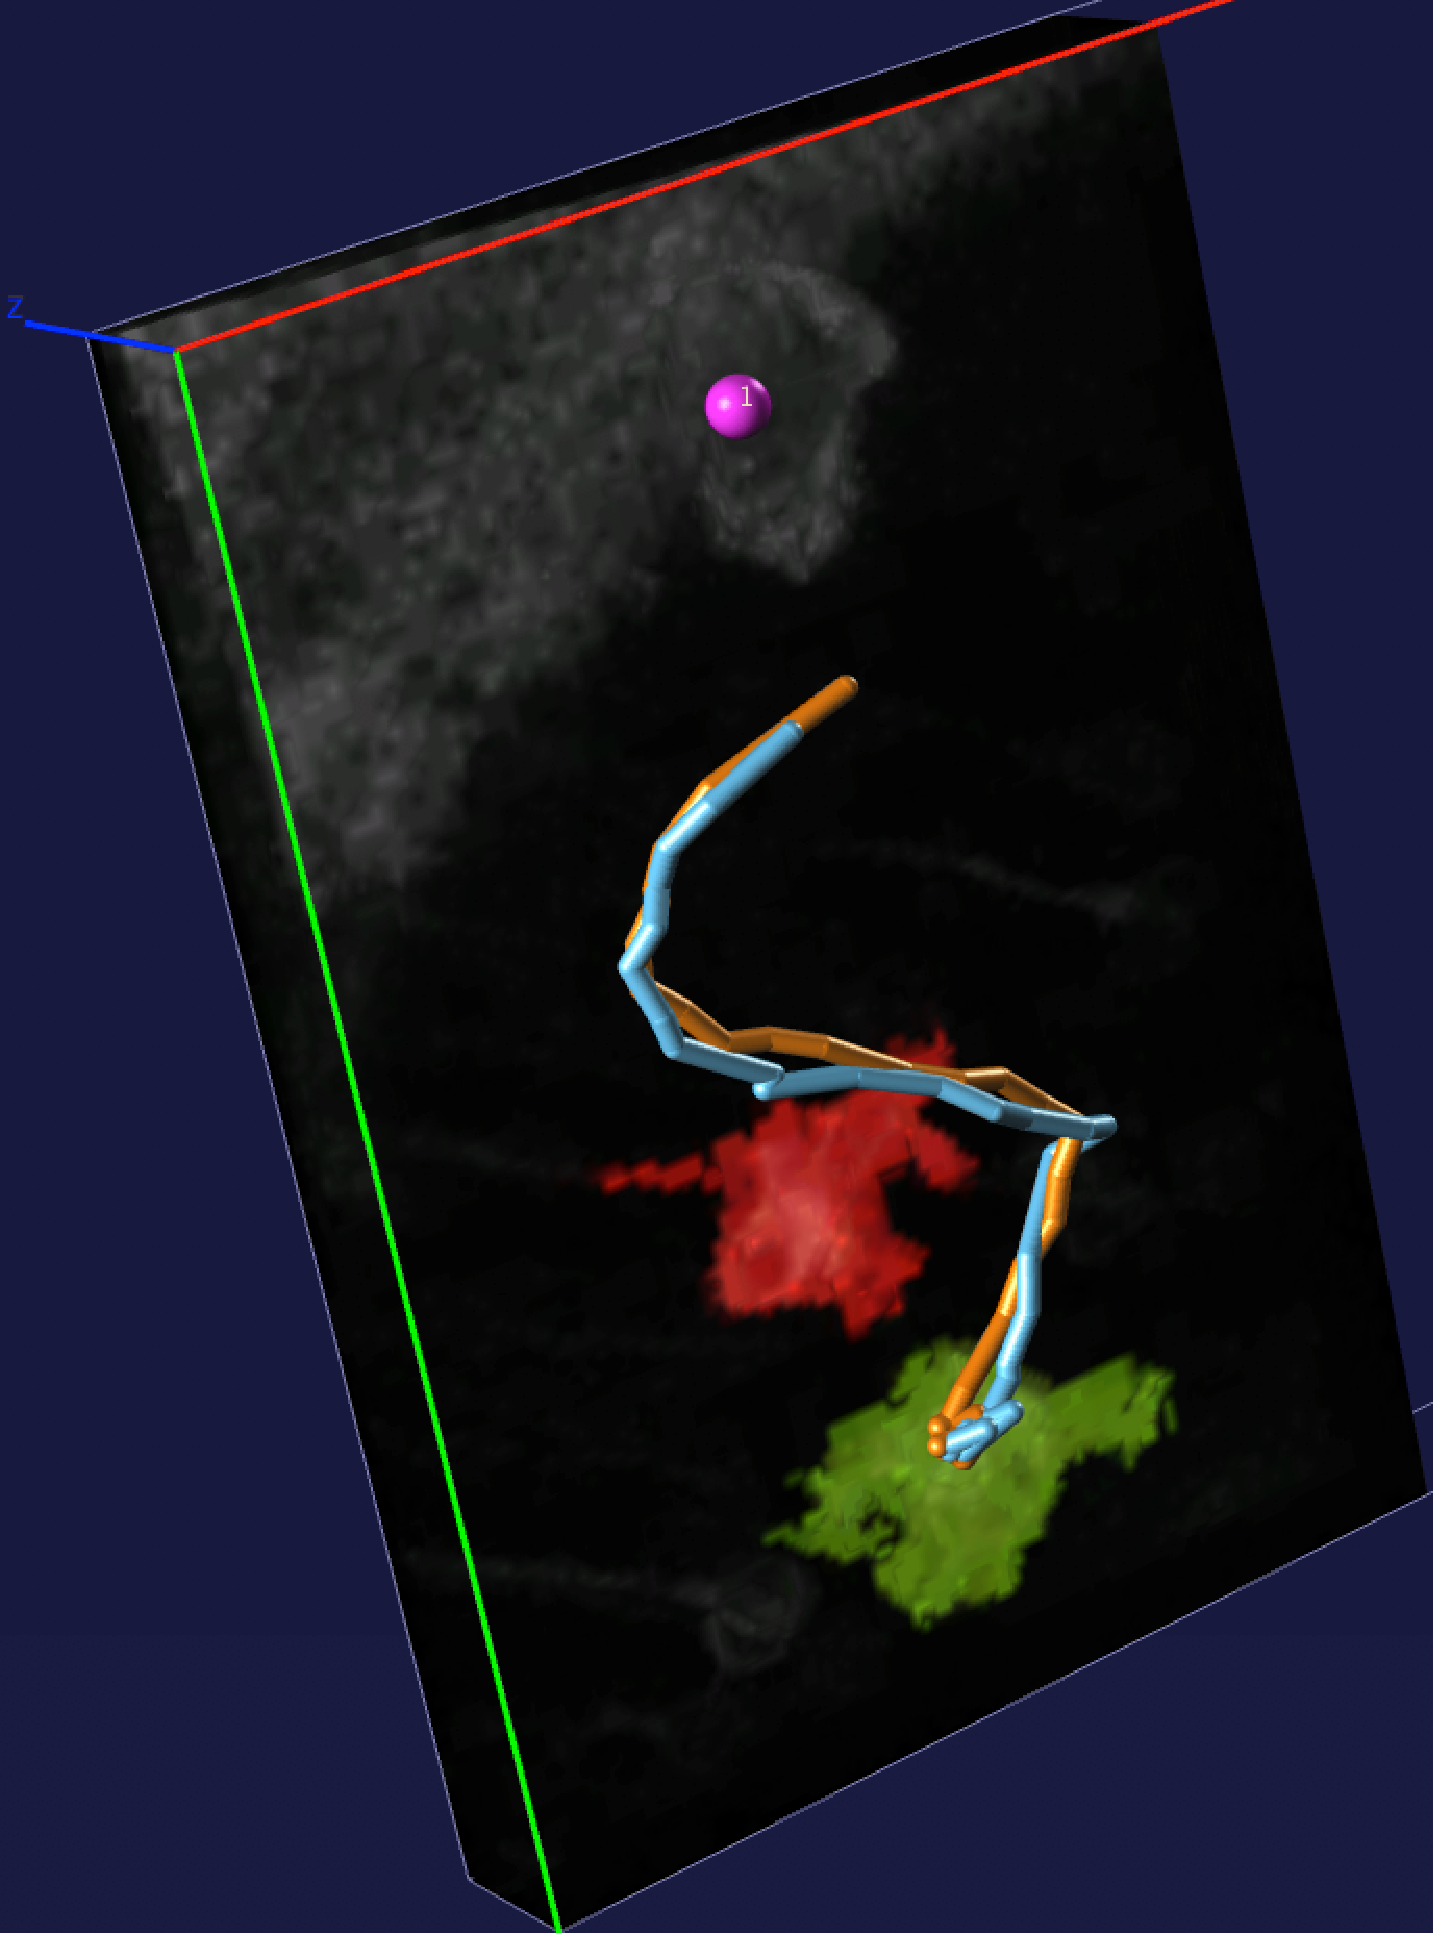
\includegraphics[width=.7\linewidth]{images/coseg_fig1}
  \caption[3D motion patterns of two microglia \textit{in vivo} 
   reconstructed using \texttt{ct3d}]{3D motion patterns of two microglia \textit{in vivo}
    reconstructed using \texttt{ct3d}.  The red and green areas
    indicate initial positions of the two microglia. While the red
    cell remains in resting state, the green cell is activated through
    an induced injury and migrates along a trajectory (orange line:
    trajectory obtained by \texttt{ct3d}; blue line: trajectory
    obtained from manual annotation) towards a site of injury (purple
    dot);}
  \label{fig:coseg-fig1}
\end{figure}

The lack of methods for tracking cells in 3D has been reported as a
limiting factor, for instance in the context of immunoimaging
\cite{Cahalan:08}. Despite the well-established protocol to capture
microglia, innate immune cells in the central nervous system, in 3D
using two-photon microscopy following the seminal works by
\cite{Nimmerjahn:05} and \cite{Davalos:05}, motility analysis has
been performed by (and limited to) manual estimations derived from 2D
projections \cite{Davalos:08} in the numerous studies following these
protocols. In fact, tracking microglia cells is complicated by several
aspects. Microglia tightly contact specific brain structures in their
resting state \cite{Wake:09}, often making it difficult to clearly
separate them from their surrounding tissue. Furthermore, the
extension and retraction of so-called microglia \emph{processes} makes
it practically impossible to separate them from other cells or
surrounding tissue in a 2D projection. As we demonstrate in this
study, cosegmentation based cell tracking may overcome these
difficulties and allows to reliably track microglia in 3D, both in
resting state and when moving in activated state, as displayed in
Figure \ref{fig:coseg-fig1}.

% Our method an related approaches: thresholding / localized /
% mutli-thresholding
From an algorithmic point of view, our method can be seen as a broad
generalization of \emph{thresholding methods}. Otsu's early and still
commonly used approach \cite{otsu1975threshold} picks a cut-off intensity based
on the gray-value histogram of an image, considering pixel intensities
below this threshold as background and pixels exceeding the threshold
intensity as foreground. To deal with background inhomogeneities and
objects of varying intensities, different approaches such as locally
adaptive thresholding \cite{Kim:05} have been developed. Our approach
utilizes a highly systematic way of picking local thresholds in a
hierarchical representation of all possible thresholds of an image,
the so-called component tree \cite{jones1999connected,Najman:04}. In order to
pick local thresholds in the component tree, we compare the component
trees of consecutive time frames by solving the so-called \emph{tree
  assignment} problem, a natural generalization of bipartite matchings
and the associated assignment problem. Comparing component trees by
computing tree assignments yields a \emph{cosegmentation} of two
images; for cell tracking, cosegmentations between two time frames in
a video sequence are of particular relevance.

While the term cosegmentation has been coined by \cite{Rother:06},
our approach significantly differs from their approach, which is based
on comparing histograms. On the contrary, our approach is
morphological in the sense that it attempts to identify overlapping
regions in two images by finding an optimal tree assignment.

Using cosegmentation has potential further applications in location
proteomics beyond the cell tracking problem investigated in this
paper. Tree assignments as a generalization of bipartite matchings
were introduced and applied by the last author recently
\cite{mosig2009tracking}, and were recently shown to be computationally hard
in general \cite{Klau:10}. Applying tree assignments to component
trees for obtaining cosegmentations is a novel contribution in this
work. In fact, cosegmentations promise to be useful in other
bioimaging (and eventually image processing) applications beyond cell
tracking. One straightforward application where cosegmentation is of
high relevance are protein-colocalization studies. Studying
colocalization has recently become of relevance through the
availability of corresponding two- or multi-label fluorescence
microscopy \cite{Zinchuk:08,Schubert:06} or in-situ hybridization
\cite{Carson:09,Boettiger:09} techniques.

We implemented our algorithm in the publicly available \texttt{ct3d}
software package, which is accompanied by the \texttt{at3d} graphical
user interface. In terms of applying our algorithm, this paper focuses
on evaluating the performance of our cosegmentation based approach for
3D cell tracking, leaving colocalization studies as a future
direction. Cell tracking performance is evaluated both on two-photon
live cell imaging data displaying zebrafish microglia \textit{in
  vivo}, and on synthetically generated data that allow to determine
the algorithm's accuracy based on the ground truth the synthetic data
were generated from.

\section{Methods}

\begin{figure}[htbp]
\centering
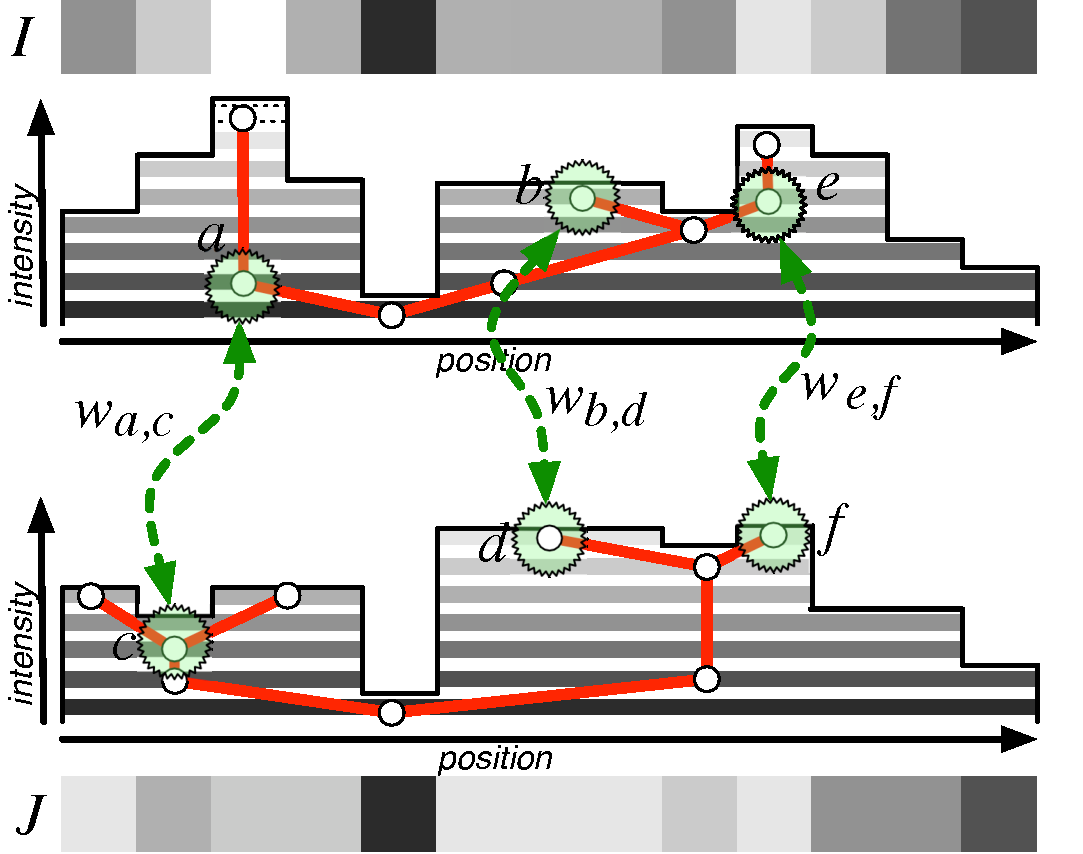
\includegraphics[width=.5\textwidth]{images/coseg_fig2}
\caption[Tree assignment of two (pruned) component trees for two 1D images I and J]{Tree assignment of two (pruned) component trees for two 1D images I and J. Vertices not eliminated by the second pruning step are indicated by circles. All other non-branching vertices are eliminated in the pruning step. The tree assignment indicated by the dashed arrows is $A = \{(a, c), (b, d), (e, f)\}$ with a weight of $w_{ac}+w_{bd}+w_{ef}$.}
\label{fig:coseg-fig2}
\end{figure}

Our algorithm is based on representing each image $F_1,\ldots,F_N$ by its component tree\cite{jones1999connected}. The component tree of an image $I$ is obtained by considering the connected components of the thresholded versions $I_θ$ of I under all possible thresholds $θ$. The set of all connected components under all thresholds is obviously hierarchically ordered by subset inclusion. This hierarchical order defines the component tree, which can be computed in linear time \cite{Najman:04}. For examples of 1D images and their component trees refer to Figure \ref{fig:coseg-fig2}. 

Figure \ref{fig:coseg-fig3} illustrates the basic steps of our cell tracking algorithm. The outline of the algorithm is as follows: we start with computing and pruning component trees for each time frame. Then, tree assignments between each pair of consecutive component trees are computed. The tree assignments can be turned into segmentations of the original images. This produces two segmentations of each image, requiring computation of a consensus segmentation. The resulting unique segmentation of each image then requires a standard bipartite matching between consecutive time frames to track cell identities over time. 

\subsection{Building component trees and tree assignment}
Details for \emph{component tree construction} and \emph{tree assignment} is introduced in Chapter \ref{chpt:cptree} and Chapter \ref{chpt:treeassign}.

\begin{figure}[htbp]
\centering
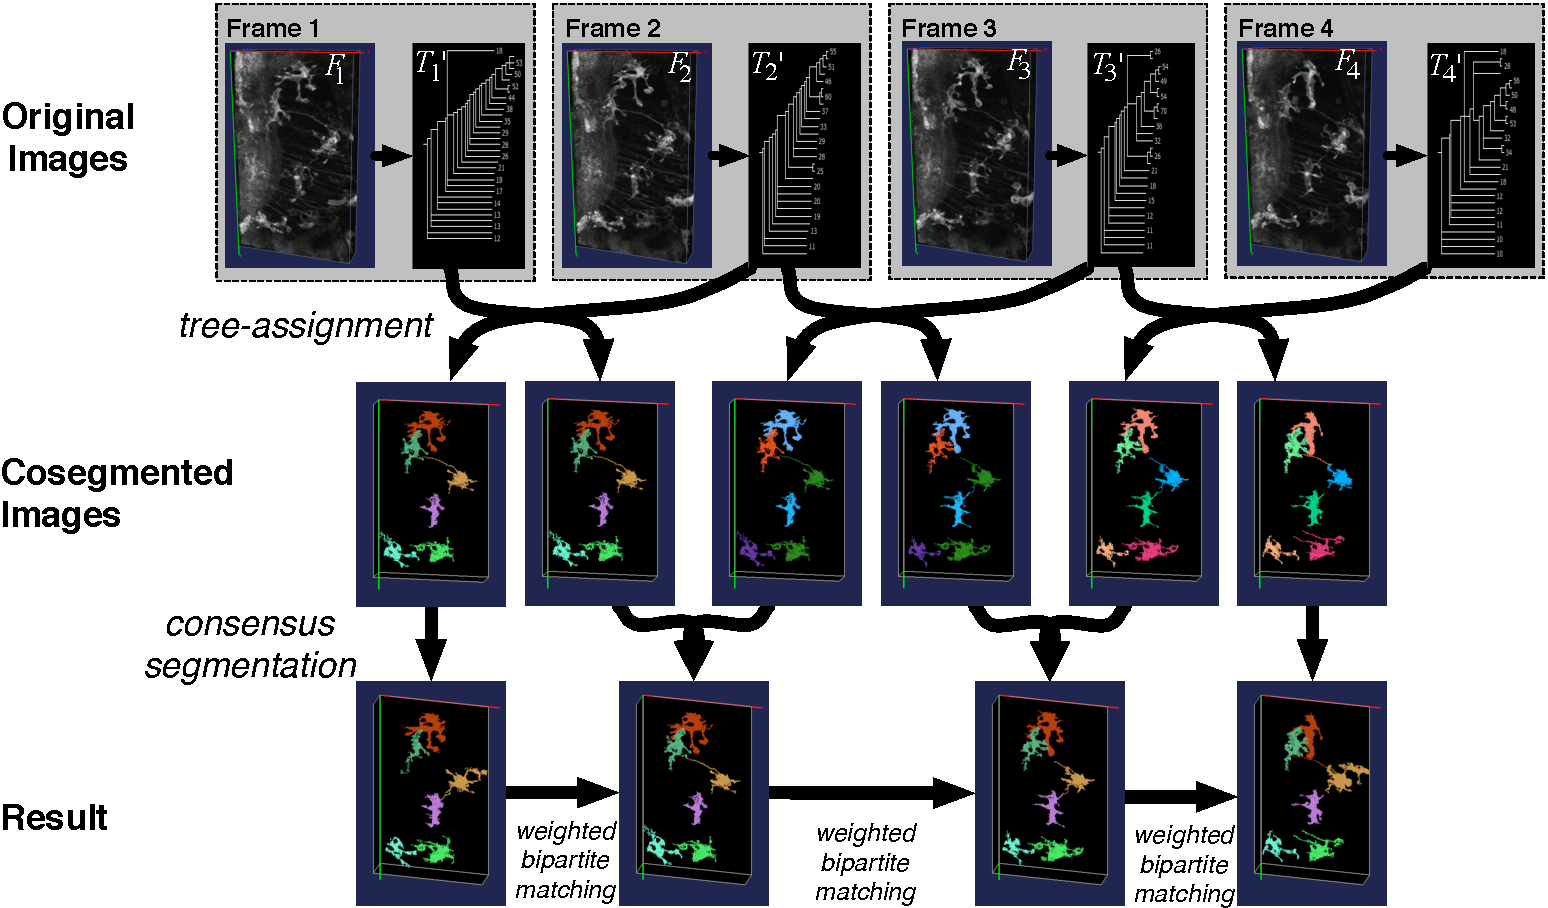
\includegraphics[width=1.0\textwidth]{images/coseg_fig3}
\caption{Overview of complete cell tracking algorithm}
\label{fig:coseg-fig3}
\end{figure}

\fbox{
\begin{minipage}{1.0\textwidth}
    {\bf Algorithm \texttt{cosegmentation-track}}
      \begin{itemize}
      \item \emph{Input:} Sequence of images $F_1,\dots,F_N$; pruning
        parameters $\theta_{\min},\theta_{\max}$, single-node cutoff
        $\sigma$.
      \item \emph{Output:} Sequence of segmented images $S_1',\dots,S_N'$.
      \end{itemize}
    \begin{enumerate}
    \item Compute component tree $T_i$ for all $i\in[1:N]$
    \item Prune $T_i$ to obtain $T_i'$ using
      $\theta_{\min},\theta_{\max},\sigma$.
    \item For each $i\in[1:N-1]$, compute
      $A_i=\mathrm{treeassign}(T_i,T_{i+1})$.
    \item Use $A_i$ and $A_{i+1}$ to obtain two segmentations of image
      $F_i$; compute consensus segmentation $S_i$ from these two.
    \item For each $i\in [1:N-1]$, compute a maximum-weighted bipartite
      matching between the segments in $S_i$ and $S_{i+1}$.
    \item Assign random color to each segment in $S_1$ to obtain $S_1'$. In $S_{i+1}'$,
      assign the same color to the segment as the one matched in $S_i$
    \end{enumerate}
  \end{minipage}
}

\subsection{Turning tree assignments into cosegments}
Assume $A=\{(a_1,b_1),\ldots,(a_k,b_k)\}$ is a tree assignment between the component trees of two images $I$ and $J$. Then the areas $\beta(a_1),\ldots,\beta(a_k)$, where $\beta(a)$ is defined in Section \ref{sec:alpha-beta-area},  refer to pairwise disjoint segments in $I$, and can hence be considered as a segmentation of $I$. Correspondingly, the areas $\beta(b_1),\ldots,\beta(b_k)$ induce a segmentation of $J$; note that the segments $\beta(a_i)$ and $\beta(b_i)$ necessarily overlap, as they require a non-zero weight to be included in an optimal tree-assignment.

\subsection{Consensus segmentation and bipartite matching}
When determining a segmentation of frame $i$, we are confronted with two competing options; one segmentation $P_i$ resulting from the cosegmentation of frames $i-1$ and $i$, the other one, $Q_i$, from the cosegmentation of frames $i$ and $i+1$. We resolve this by computing a consensus segmentation. We generally use $P_i$ as the starting point of a consensus segmentation. Any segment in $Q_i$ that does not overlap with any segment $P_i$ is supplement to $P_i$ to obtain the consensus segmentation $P_i′$. This ensures that cells entering the scene in frame $i$ can be identified in frame $i$ (rather than frame $i+1$).

\subsection{Filtering results}
As for most segmentation and tracking approaches, the results obtained from the steps described above has a tendency toward overdetection, i.e. detecting segments that result from image noise rather than cells. To filter out those segments, we utilize life span filtering, i.e. we filter out all cells whose identity can be traced across less than a certain minimum number of frames. This cell filter, along with several other ways to eliminate cells with unsuitable size or volume features, follows corresponding features of the Celltrack software \cite{sacan2008celltrack} for 2D cell tracking; for ct3d, they are implemented in the graphical user interface of the at3d tool shown in Figure \ref{fig:coseg-fig4}.

\begin{figure}[htbp]
\centering
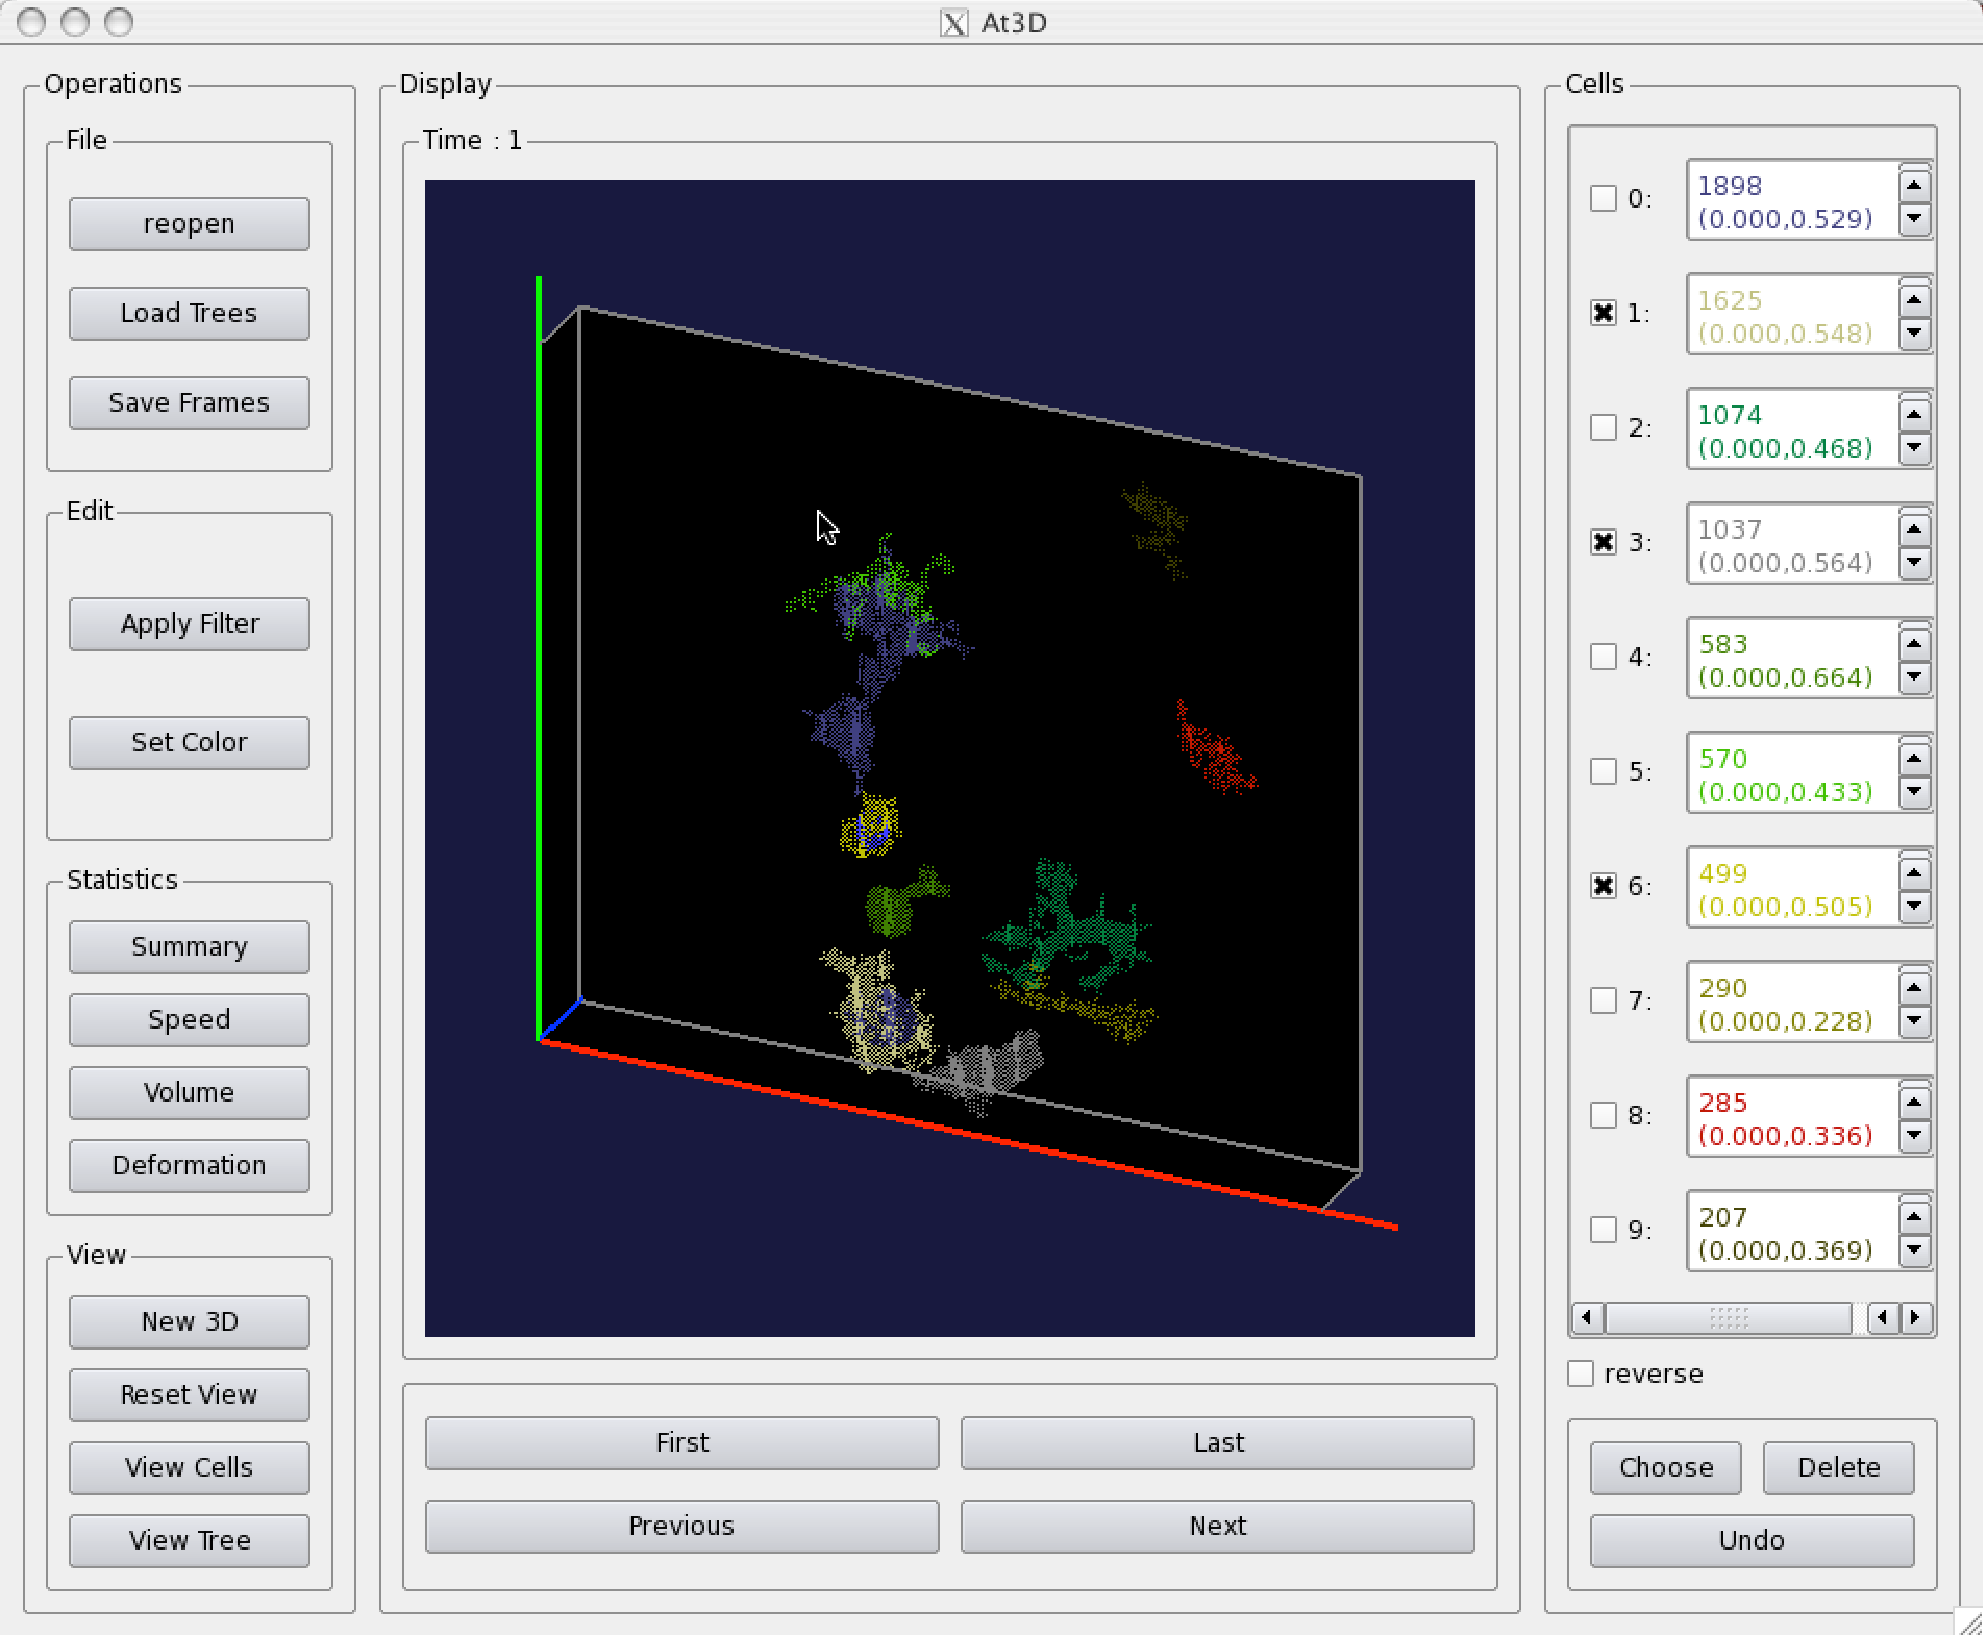
\includegraphics[width=.5\textwidth]{images/coseg_fig4}
\caption[Screenshot of at3d]{Screenshot of at3d, which is designed for exploring cell tracking results and extracting motility parameters. It also supports features for correcting overdetection and oversegmentation. Cells can be selected and removed either individually or by filtering based on different criteria such as size or life span.}
\label{fig:coseg-fig4}
\end{figure}

\section{Implementation}
We implemented component trees, tree-assignments and the complete cell tracking algorithm, in C++ using lp\_solve\footnote{http://lpsolve.sourceforge.net/5.5/} for solving both the tree assignment and the weighted bipartite matching (integer) linear programs, all of which is compiled in the ct3d command line tool. Cell tracking results can be further explored using at3d, which allows the user to select and extract specific cells identified by the cell tracking procedure, and derive their motility parameters such as velocity and deformation. The at3d tool is implemented using the qt framework for graphical user interfaces. Input and output of image series is designed to be compatible with other visualization software, most notably v3d \cite{peng2010v3d} for producing rendered visualizations of the output.
\section{Experimental materials and methods}

3D time-lapse two-photon microscopy imaging of zebrafish microglia was
performed as follows: \emph{Zebrafish preparation}. Zebrafish
\emph{Tg(ApoE:egfp)}, in which microglia express EGFP \cite{Peri:08},
were maintained in the National Zebrafish Resources of China (NZRC,
Shanghai, China) with an automatic fish housing system (ESEN, Beijing,
China) at 28$^{\circ}$C. Embryos were raised at 28.5$^{\circ}$C under
a 14/10 hour light-dark cycle in 10\% Hank’s solution, which consists
of (in mM) 140 NaCl, 5.4 KCl, 0.25 Na2HPO$_4$, 0.44 KH$_2$PO$_4$, 1.3
CaCl$_2$, 1.0 MgSO$_4$ and 4.2 NaHCO$_3$ (pH 7.2). They were staged as
previously described \cite{Kimmel:95}. Zebrafish handling procedures
were approved by Institute of Neuroscience, Shanghai Institutes for
Biological Sciences, Chinese Academy of Sciences.

\emph{Time-lapse imaging.} For \textit{in vivo} imaging, zebrafish
larvae at 5-7 days postfertilization (dpf) were first anesthetized
with Hank’s solution containing 0.02\% tricaine methanesulfonate
(MS222) and embedded in 1.5\% low-melting point agarose. Time-lapse
images of microglia were captured, via a 40X water objective mounted
on a two-photon microscope with 900 nm (Prairie) or a Nikon A1R
confocal microscope with 488 nm. Z-stack images, which covered the
whole area of microglia in the optic tectum, were collected every 2
min at a section thickness of 1 $\mu$m. Each frame (512$\times$512
pixels, 14 to 34 Z-stack images) was averaged 4
times.

\section{Results}
\label{sect:results}

We evaluated our algorithm on two types of data. First,
   we applied it to an \textit{in vivo} time-lapse sequence of 3D
   two-photon images of zebrafish midbrain, displaying the motility of
   microglia; second, we applied \texttt{ct3d} to synthetically
   generated data for quantifying the accuracy of our cell tracking
   results.

  Evalutation on \textit{in vivo} data was accomplished by comparison
  with manually annotated trajectories of specific microglia in three
  data sets. Note that manual annotation is limited to trajectories,
  whereas boundaries of the cell volumes are almost impossible to
  obtain in 3D, beside systematic problems with manual annotations
  \cite{Huth:10}. Hence, we additionally created synthetic ground
  truth data to further evaluate the performance of our method. We
  followed the procedure used in \cite{dufour2005segmenting}, generating (noise
  perturbed) elliptical objects of average intensity $I_o$ above
  Poisson distributed background noise of intensity $I_b$. In addition
  to the procedure from \cite{dufour2005segmenting}, we created perturbed images
  with different types of background inhomogeneities, as shown in
  Figure \ref{fig:coseg-fig5}: in a second set of data, we
  introduced a multiplicative \emph{vignetting} effect to the data,
  following the vignetting model by \cite{kang2000can} under different
  focal lengths $f$ and off-axis illumination parameters $\alpha$. In
  a third set of data, we introduced an additive linear gradient along
  the $x$-axis of different slopes $\beta$. Each time series consists
  of 20 time frames, each of size $200\times 200\times 40$ pixels. On
  these data, we ran \texttt{ct3d} with size cutoffs
  $\theta_{\min}=500$ and $\theta_{\max}=5000$, and a single-node
  cutoff of $200$ pixels. In the resulting sequences, all cells whose
  identity could be traced through the complete sequence were kept,
  while all other cells were discarded using the \texttt{at3d} tool.


\subsection{Evaluation on synthetic data}

Our results on the synthetically generated image sequences are
summarized in Table \ref{tab:coseg-tab1} and indicate that
\texttt{ct3d} is highly robust against different types and intensities
of background inhomogeneities. The results suggest that \texttt{ct3d}
has a tendency to identify components slightly (about 10\%) larger
than the actual objects. This is a natural consequence of pruning the
component trees, where the vertex that would perfectly represent an
object is unlikely to be part of the pruned tree. This effect can be
reduced by smaller choice for the single-node cutoff parameter
$\sigma$ at the cost of higher computation time.

\begin{table*}
  \caption{Tracking results for synthetic data. }
  \centering
	\footnotesize
  \begin{threeparttable}
  \begin{tabular}{|c|ccc|rrr|rrr|}
\hline
&
\multicolumn{3}{|c}{\emph{Data Set}} &
\multicolumn{3}{|c}{\emph{\texttt{ct3d} Tracking Result}} &
\multicolumn{3}{|c|}{\emph{Chan-Vese Result}} \\\hline
&$I_o$ & $I_b$ &\emph{inhomogeneity}&\#cells&voxel recall& error rate            &\#cells         &voxel recall  & error rate\\\hline
\multirow{3}{*}{\begin{sideways}\emph{none\,\,\,\,\,\,}\end{sideways}}
& 2    & 1     & -                  & 3.00  & 99.94\%    &        9.86\%         &3.00	& 92.94\%	& 7.07\%\\	
& 3    & 1     & -                  & 3.95  & 100.00\%   &       22.93\%         &3.00	& 99.25\%	& 0.75\%\\	  
& 3    & 2     & -                  & 3.00  & 100.00\%   &       11.48\%         &3.00	& 90.25\%	& 9.75\%\\	
& 6    & 1     & -                  & 3.00  & 100.00\%   &        9.74\%         &3.00	& 99.70\%	& 0.30\%\\	
& 10   & 1     & -                  & 3.00  & 99.11\%    &       10.05\%         &3.00	& 99.93\%	& 0.07\%\\	
\hline\multirow{3}{*}{\begin{sideways}\emph{linear\,\,\,\,\,}\end{sideways}}      	  		  		
& 3    & 1     & $\beta=2$          & 3.00  & 100.00\%   &       10.62\%         &2.80	& 80.26\%	& 19.95\%\\	
& 3    & 1     & $\beta=3$          & 3.00  & 100.00\%   &        4.51\%         &2.10	& 62.97\%	& 39.00\%\\	
& 3    & 2     & $\beta=3$          & 3.00  & 99.97\%    &        6.83\%         &1.95	& 58.27\%	& 42.76\%\\	
& 6    & 1     & $\beta=3$          & 3.00  & 100.00\%   &        1.27\%         &2.20	& 66.54\%	& 41.26\%\\	
\hline\multirow{3}{*}{\begin{sideways}\emph{vignetting\,\,}\end{sideways}}        	  		  		
& 2    & 1     & $f=100,\alpha=5e-3$& 3.00  & 98.42\%    &        8.13\%         &0.85	& 22.89\%	& 77.25\%\\	
& 2    & 1     & $f=200,\alpha=1e-3$& 3.00  & 99.96\%    &        9.08\%         &1.90	& 56.56\%	& 43.60\%\\	
& 2    & 1     & $f=200,\alpha=5e-3$& 3.00  & 98.45\%    &        6.80\%         &0.60	& 15.76\%	& 84.31\%\\	
& 3    & 1     & $f=200,\alpha=1e-3$& 3.00  &100.00\%    &       14.25\%         &3.00	& 93.70\%	& 6.33\%\\	
\hline
  \end{tabular}
\begin{tablenotes}
\footnotesize
\item To assess the quality
    of tracking results, we derived the number of identified cells, the
    \emph{voxel recall}, i.e., what percentage of all ground-truth
    object voxels was recovered in the tracking result, as well as the
    \emph{error rate} defined as the ratio between the cardinality of 
    the symmetric difference between tracking result and ground truth 
    and the total number of voxels in the ground truth dataset. 
\item \emph{Left columns:} Each
    dataset displayed three cells with different intensities $I_o$ above
    different levels of noise $I_b$, displaying different types of
    background inhomogeneities (see text). 
\item \emph{Middle Columns:} The
    three cells were correctly recovered under all settings by
    \texttt{ct3d}. 
\item \emph{Right Columns:} Segmentation using the active 
    contour approach by \cite{chan2001active} is highly reliable in the absence of 
    background inhomogeneity.
    With increasing level of inhomogeneity, voxel 
    recall decreases, while the error rate increases.
\end{tablenotes}
  \end{threeparttable}
  \label{tab:coseg-tab1}
\end{table*}

Running times varied between roughly 4 and 6 minutes, with an average
of $303.42$ seconds, for completely tracking one dataset. The majority
of running time was spent on constructing the component trees and
computing the overlap weights ($14.23$ seconds on average per time
frame), whereas each tree assignment required less than one second on
average; the pruned component trees typically comprised a few dozens
of vertices.

As a reference algorithm to compare the performance of \texttt{ct3d}
against, we computed a segmentation of each time frame using the
active contour approach by \cite{chan2001active}\footnote{Results were
  computed for parameters $\mu=1$, $\nu=.7$, $\lambda_1=1$,
  $\lambda_2=2$, $\Delta t=.8$ running 100 iterations.}, which is a
well-established and state-of-the-art representative of the large
family of level set methods. As shown in Table
\ref{tab:coseg-tab1}, this method works highly accurate in the
absence of background inhomogeneity while getting less reliable with
increasing levels of background inhomogeneity, as can be expected due
to the involvement of a global background model.

\begin{figure}[htbp]
\centering
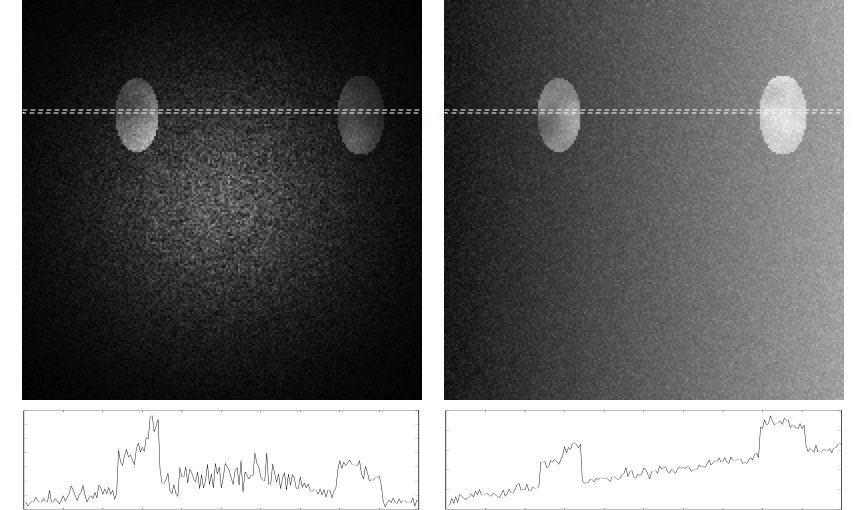
\includegraphics[width=1.0\textwidth]{images/coseg_fig5}
\caption[Sections of synthetically generated images]{Sections of synthetically generated images—Left: 2D section (top) of an image perturbed background vignetting following the Kang–Weiss model\cite{kang2000can}. The dashed box indicates the position of the 1D section displayed in the lower part. Right: same setting with the background perturbed by an additive linear gradient. In both instances, ct3d yields reliable tracking results (see Table \ref{tab:coseg-tab1}).}
\label{fig:coseg-fig5}
\end{figure}

\begin{figure}[htbp]
\centering
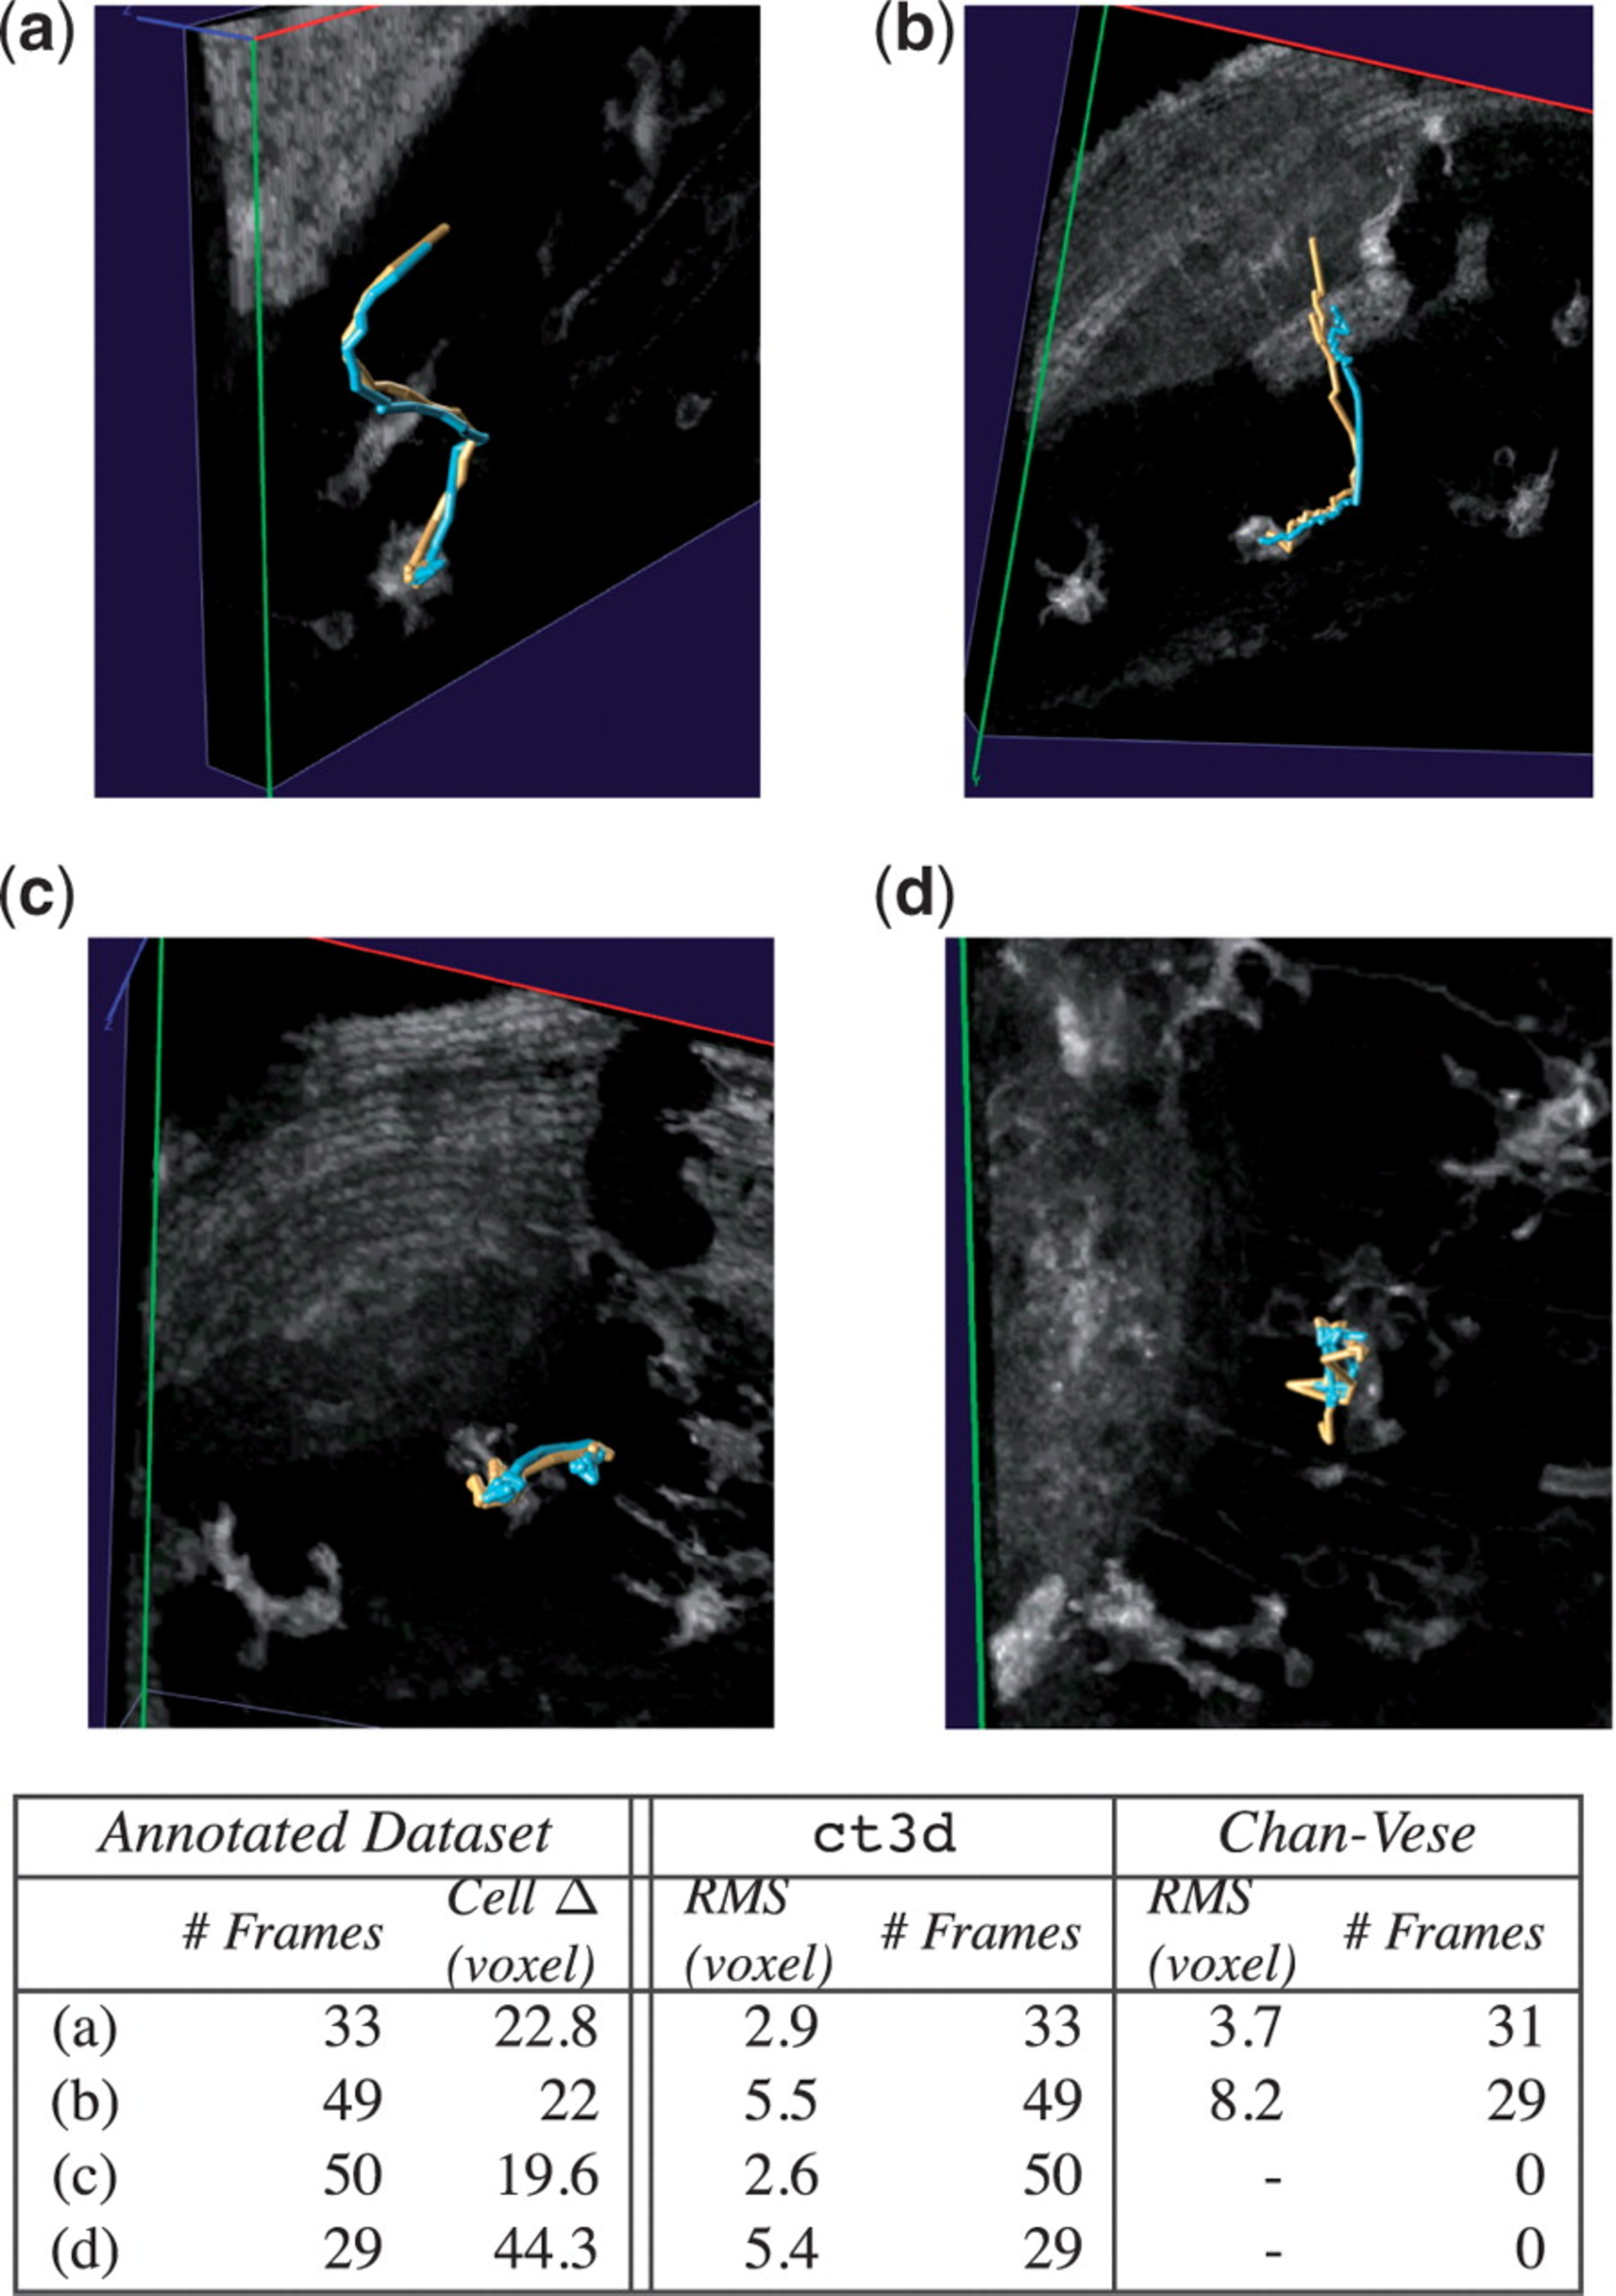
\includegraphics[width=0.6\textwidth]{images/coseg_fig6}
\caption[Cosegmentation results comparison with other methods]{Top: visualization of trajectories obtained by manual annotation (blue lines) with trajectories obtained using ct3d (orange lines) for microglia in activated state, see (a) and (b), as well as resting state, see (c) and (d). Bottom: quantitative comparison of trajectories obtained by ct3d and the active contour approach from Chan and Vese \cite{chan2001active}. In general, ct3d could identify the annotated cells in all time frames. The root mean square distance to the annotated trajectory measures a fraction of the diameter of the annotated cell (columns cell $\Delta$ and RMS), while the Chan–Vese algorithm missed varying numbers of cells or failed completely (last column). For the Chan–Vese results, a parameter set was optimized for dataset (a). This parameter set ($\mu$=1, $\nu$=.5, $\lambda_1$=.2, $\lambda_2$=5) was also applied to datasets (b) to (d). While for dataset (a), the result is comparable to ct3d, the annotated cell was identified in only 29 out of 49 time frames in (b). In datasets (c) and (d), the annotated cell could not be identified at all using these parameters.}
\label{fig:coseg-fig6}
\end{figure}
\subsection{Tracking microglia \textit{in vivo}}

Figure \ref{fig:coseg-fig6} shows a result obtained from
our tracking algorithm on a time series of microglia images measured
as described above. We reduced resolution by half, so that the
resulting width and height varied between 146 and 250 pixels, while
the depth ranged between 14 and 66 layers for each time frame; each
time series comprised 30 to 80 time frames. Gray scale resolution was
reduced from 16 bit to 8 bit. We applied \texttt{ct3d} using
parameters $\theta_{\min}=200$, $\theta_{\max}=10,000$ and a
single-node cutoff of $200$ pixels; the resulting pruned component
trees contained 69 vertices on average, ranging between 40 and 168
vertices. Running times varied between roughly 2 to 10 minutes, with
471 seconds on average. 

Under the given experimental protocol, the phenomenon of
\emph{overdetection}, i.e. the recognition of segments that are not
microglia, is inevitable. This is due to the limited specificity of
the \emph{apoE-GFP} gene, which is also expressed in cells other than
microglia in the surrounding tissue, often at comparably high levels
as in microglia. Yet, \texttt{ct3d} identifies microglia as segments
that can be visually distinguished from non-microglia segments by a
human observer due to their characteristic shape or motion
patterns. The graphical user interface of the \texttt{at3d} tool (see
Figure \ref{fig:coseg-fig4}) allows to manually eliminate false positive
cells from tracking results by different filtering and visual
selection functions similar to those provided by \texttt{Celltrack}
for two dimensional time lapse sequences. The \texttt{at3d} tool also
allows to manually correct for the occasionally observed events of
oversegmentation, i.e., one microglia being recognized as two segments.

We used \texttt{at3d} to eliminate non-microglia from all six datasets
and correct oversegmentation in individual frames. We were able to
reconstruct trajectories of all relevant microglia that can be
visually identified in the original datasets; only one dataset was
affected by a sudden ``frameshift'', i.e., the sample changing its
distance to the camera in the $z$ direction, leading to interrupted
trajectories at the corresponding time frame. In few other cases, the
trajectory of a microglia was interrupted in individual frames, which
we could correct using \texttt{at3d}.

In order to quantitatively evaluate the quality of \texttt{ct3d}
results on \textit{in-vivo} microglia data, we compared \texttt{ct3d}
trajectories with manual annotations. To this end, we selected four
microglia from four different datasets and annotated their
trajectories manually using the 3D polyline markup feature of the
\texttt{v3d} software. The root mean square distance between the
\texttt{ct3d} and the manual trajectories turned out to be 2.9 voxels,
5.5 voxels, 2.6 voxels, and 5.4 voxels, respectively, in the four
different datasets. These deviations can be considered relatively
small in relation to the cell diameters, which were measured as 22.8,
22, 19.6, and 44.3 voxels, respectively.

We also applied the active contour approach from \cite{chan2001active} to
the datasets. Identifying the the four microglia in our annotated
evaluation dataset required intensive tuning of the four major
parameters. In fact, we could not identify a single set
  of parameters that works across all datasets. A parameter set tuned
  for a specific dataset worked comparably well on the respective
  dataset, but performed significantly worse or yielded no result on
  other datasets, see Fig. \ref{fig:coseg-fig6}.

\section{Discussion}

We have presented a novel approach to tracking cells in three
dimensional time lapse microscopy image sequences, based on the
concepts of component trees and cosegmentation. We demonstrate that
this approach is robust against the numerous challenges imposed by
images measured in an \textit{in vivo} environment, and allows to
identify microglia and their motion patterns in zebrafish neural
tissue when combined with the \texttt{at3d} annotation tool. In a
quantitative evaluation, we show that our approach is robust against
different types of background inhomogeneities. This suggests that
\texttt{ct3d} and \texttt{at3d} are potentially useful for \textit{in
  vivo} imaging studies investigating other aspects than just
microglia motility. In its current formulation, our cosegmentation
approach relies on the assumption that the area occupied by an object
overlaps between two consecutive time points. While this may not be
satisfied in all cell tracking problems (e.g. when tracking
centrosomes \cite{Jaensch:10}), it is a reasonable assumption for
many immunoimaging related studies.

To the best of our knowledge, our approach is the first that can
identify and track microglia in live cell imaging time series. In most
cases, obtaining reliable trajectories still requires manual
post-processing of the output. The most notorious difficulties
certainly are the complex morphology -- their deformation patterns,
irregular shapes, and interaction with the surrounding -- as well as
the unspecificity of the fluorescent markers available. In this light,
our approach constitutes significant progress in the sense that it has
sufficient sensitivity to separate microglia form their
surrounding. Yet, a fully automated approach remains a major and
certainly non-trivial challenge. A first step in this direction might
be the combination with level-set based approaches as utilized for 2D
cell tracking by \cite{Nath:06} that might yield more accurate cell
boundaries in some cases. Yet, \texttt{ct3d} promises to be a key tool
for further studying open questions regarding microglia, such as to
determine if and how glia and microglia share the task of finding and
removing apoptotic neurons from the vertebrate brain \cite{Peri:08}. 

Beside the direct relevance for \textit{in vivo} time lapse
microscopy, our study indicates that our morphological approach to
cosegmentation is both practical and of relevance in
bioimaging. Consequentially, it appears a natural approach to apply
cosegmentation to protein colocalization studies, which have attracted
considerable attention in recent years following the availability of
two- or multi-label fluorescence microscopy \cite{Zinchuk:08}.

Another major experience that can be drawn from our work is the obvious
potential of component trees and the closely connected theory of
component filters in bioimaging. While component filters are well
known to leave relevant gradients unchanged, recent work such as the
results by \cite{Coupier:05} allow to assign a
statistical significance to components observed in an image. Such
concepts might be particularly useful when combining component trees
with cosegmentation for judging the relevance of colocalized segments
observed when comparing two component trees.

\section{Contribution of this thesis}
In this thesis, we build a cosegmentation based pipeline for 3D time-lapse microglia cell tracking.
The novel cosegmentation methods accomplish cell segmentation and cell association simutaneously through 
component tree assignment. We evalute our method on synthetically generated data, demonstrating that our algorithm is robust even in the presence of different types of inhomogeneous background noise. Our algorithm is implemented in the ct3d package, which is available under http://www.picb.ac.cn/patterns/Software/ct3d.
